%        File: additional_info.tex
%     Created: Fri Jul 19 04:00 PM 2013 C
% Last Change: Fri Jul 19 04:00 PM 2013 C
%
\documentclass[a4paper]{spie}
\usepackage[]{amsmath}
\usepackage[detect-all]{siunitx}
\usepackage{textcomp}
\usepackage{booktabs}
\usepackage[affil-it]{authblk}
\usepackage[]{graphicx}
\usepackage{subcaption}
\usepackage{tikz}

\graphicspath{{figures/}}
\newcommand{\de}[1]{\ensuremath{\operatorname{d}\!{#1}}}

%fix path issue with png files
\let\pgfimageWithoutPath\pgfimage 
\renewcommand{\pgfimage}[2][]{\pgfimageWithoutPath[#1]{figures/#2}}

\begin{document}
\title{Performance of X-ray grating interferometry at high energies}
\author{Matteo Abis, Thomas Th\"uring and Marco Stampanoni}
\affil{ETH Z\"urich and Paul Scherrer Institut}
\renewcommand{\today}{}
\maketitle
\begin{abstract}
A theoretical description of the performance of a Talbot and Talbot-Lau
type interferometers is developed, providing a framework for the
optimization of the geometry for monochromatic and polychromatic
beams. Analytical formulas for the smallest
detectable refraction angle and the visibility of the setup are derived.
The polychromatic visibility of the interference fringes is particularly
relevant for the design of setups with conventional X-ray tubes, and it
is described in terms of the spectrum of the source and the type of
beam-splitter grating.
We show the practical realization of such a design by imaging a metallic
screw at~\SI{100}{\kilo\eV}.
\end{abstract}

\section{Grating interferometry}
Grating interferometry (figure~\ref{interferometer}) is an imaging technique yielding complementary
signals from the interaction of X-rays with matter. Besides the absorption
image, a phase shift~\cite{David2002,Momose2003a} and a
scattering~\cite{Pfeiffer2006} signal
can be simultaneously retrieved from the interference pattern.

This approach does not rely on a highly coherent source, thus it can be applied
to ordinary X-ray sources and not only to synchrotron facilities.
The fundamental principle of this interferometric device is the Talbot
self-imaging effect, where an image of a phase grating G1 is formed
at certain distances downstream of the grating itself.

The phase sensitivity is given by the lateral displacement of the fringes in this
interference pattern, corresponding to phase variations introduced by a
sample in the direction $x$, perpendicular to the grating lines. The
refraction angle $\alpha$ is then:
\begin{equation*}
    \alpha = -\frac{1}{k} \frac{\partial\varphi}{\partial
    x}.
\end{equation*}

However, this displacement is so small for X-rays that the period of the fringes
needs to be in the micrometer range. These fringes would not be visible
at the resolution of typical medical imaging detectors. For this reason, an
analyzer grating G2 with the same period as the interference pattern is
installed in front of the detector. By scanning G2 along the $x$ direction, the convolution between
the interference pattern and the transmission profile of the grating itself
is recorded on each pixel, yielding a \emph{phase stepping curve}.
Three parameters can be extracted by comparing the curve with the sample
with a flat field image: the average value, related to the
conventional absorption, the phase displacement, and the amplitude, which
depends on the scattering~\cite{Wang2009}.

Finally, a grating interferometer can be set up on spatially incoherent and
polychromatic sources, provided that a third grating G0 is introduced close
to the X-ray tube~\cite{Pfeiffer2006,Chen2010a,Momose2009a}. This setup is
known as a Talbot-Lau interferometer, where the source grating
creates an array of individually coherent but mutually incoherent sources
whose interference patterns are superimposed on the detector.

\begin{figure}[h]
    \centering
    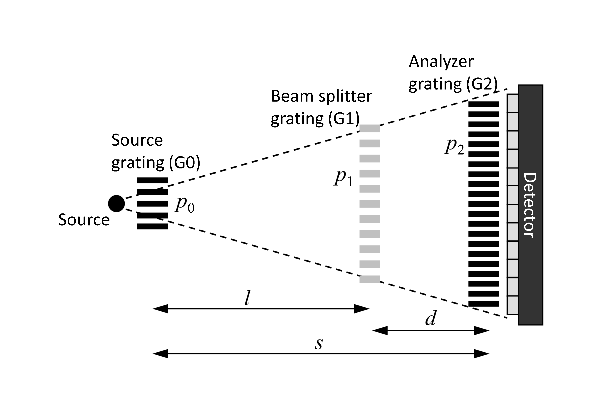
\includegraphics[width=0.5\textwidth]{grating_interferometer.eps}
    \caption{Parameters of a grating interferometer. The Talbot
    interferometer does not include a source grating G0.}
    \label{interferometer}
\end{figure}

In order to achieve maximum performance, the design parameters of the
interferometer, such as the pitch of the gratings and their position have to
be tuned. 

\section{Sensitivity optimization}
The fundamental parameter for the optimization of the geometry is the
sensitivity, or smallest detectable refraction angle, given
by~\cite{Raupach2011}:
\begin{equation*}
    \sigma_\alpha = \frac{p_2}{\pi d}
    \frac{\sqrt{2}}{v}\sigma_{\text{det}},
\end{equation*}
where $v$ is the visibility of the fringes, defined in this work as the
ratio between the magnitudes of the first and zeroth Fourier coefficients of
the phase stepping curve, and $\sigma_{\text{det}}$ is the
tipically poissonian noise introduced by the detector.
The minimization of the smallest detectable refraction angle 
$\alpha_\text{min}$\cite{Thuering2012} for a Talbot intereferometer is
achieved in two steps.
The smallest source sizes $w$ and analyzer grating periods should be chosen,
according to the properties of the X-ray tube and the available grating
technology. Then, an optimum period $p_{1}$ of the beam-splitter grating can be
calculated by minimizing $\sigma_\alpha$.

It can be shown that this is equivalent, for a $\pi$-shifting phase grating,
to minimizing~\cite{Thuering2014}
\begin{equation*}
    \sigma_\alpha \propto \frac{2p_2}{2p_2 - p_1}e^{\pi w
        \frac{2p_2 - p_1}{p_1 p_2}}.
\end{equation*}

For the Talbot-Lau design, on the other hand, the smallest $\sigma_\alpha$ is achieved for
the smallest sum of the pitches of G0 and G2
This is because the factor $\sigma_\alpha \propto p_2/d$ can be rewritten,
for a fixed total length $s$:
\begin{equation*}
    \frac{p_2}{d} = \frac{p_0 + p_2}{s}.
\end{equation*}                              
This ratio is limited by
the grating fabrication. Since the process is the same for both the source
and analyzer grating, this leads to the constraint $p_0 = p_2$, and a 
symmetric setup is the most sensitive.
                                             
\section{Optimizing the data analysis}
The analysis of the phase stepping curves is usually performed with Fast Fourier
Transform algorithms applied to the phase steps recorded as G2 is displaced
in front of the interference pattern.
The first Fourier coefficient is then the absorption, the angle of the first
coefficient is the phase displacement and the magnitude of the first
coefficient is the amplitude of the curve.
This algorithm is mathematically equivalent to an unweighted least squares fit~\cite{FFTEquivalence}.

With a more computationally intensive procedure, each point can be weighted
with the inverse of the poissonian variance given by the detector.

\begin{figure}[htb]
    \centering
    \begin{subfigure}[b]{\textwidth}
    \centering
    \input{figures/stats_phase_visibility_sd.pgf}
    \caption{}
    \label{fig:stats_phase_visibility_sd}
    \end{subfigure}
    \begin{subfigure}[b]{\textwidth}
    \centering
    \input{figures/stats_visibility_visibility_sd.pgf}
    \caption{}
    \label{fig:stats_visibility_visibility_sd}
    \end{subfigure}
    \caption[Variance of the parameters of the phase stepping curves.]{
        Comparison of the standard deviation of the
        phase~(\ref{fig:stats_phase_visibility_sd}) and
    amplitude~(\ref{fig:stats_visibility_visibility_sd}) given by the
    Poisson variance in the detected number of hits for each phase stepping
    point.}
\end{figure}
\begin{figure}[htb]
    \centering
    \input{figures/stats_visibility_visibility_mean.pgf}
    \caption[Bias of the amplitude estimator for low exposure times.]{Bias
    of the reconstructed visibility for low detector counts.}
    \label{fig:stats_visibility_visibility_mean}
\end{figure}
These two algorithms are compared through the simulation of sinusoidal phase
stepping curves with nine steps each and purely poissonian noise $\sigma_i =
\sqrt{N_i}$, where $N_i$ is the number of counts for point $i$.
To obtain statistically significant results, \num{100000} curves for each mean
value and visibility are generated.

The results of the statistical analysis of the simulation in
figure~\ref{fig:stats_phase_visibility_sd} show the standard deviation of
the reconstructed phase value as a function of visibility and for three
values of the average intensity, which is proportional to the exposure
time. For low visibilities, the poissonian weights are not very different
for different phase stepping points. Thus the weighting does not improve
the fit. The weighted estimators have minimum variance
among all the linear estimators by the Gauss-Markov
theorem~\cite{eadie2006statistical} and a real difference appears for
visibilities above \SI{50}{\percent}, which could only be reached in synchrotron
experiments. This result could also be useful if other sources of noise can
be determined, such as source instabilities.

On the other hand, the variance of the
visibility~(figure~\ref{fig:stats_visibility_visibility_sd}) does not depend
strongly on the visibility itself, but is inversely proportional to the
exposure time. It is important to not here that, for very
low counts, which occur for short exposure times or in areas with very high
absorption, the visibility is
biased~(figure~\ref{fig:stats_visibility_visibility_mean})~\cite{Chabior2011}.
This occurs for both the weighted and unweighted fit algorithms.

These results show that the increased computational complexity of the
weighted least squares fit can not be justified for experiments with lab
sources, which can not reach a visibility above \SI{50}{\percent} because of
the low temporal coherence.

\section{Experimental results}
The results of these theoretical calculations have been used
in the design of a Talbot-Lau interferometer for a high-energy X-ray tube
(160 kVp) at the Paul Scherrer Institute (Switzerland).

The design energy of the interferometer is $E_0 = \SI{100}{\kilo\eV}$, and the first
Talbot distance was used to achieve the maximum spectral
acceptance~\cite{Weitkamp2005}. The setup is then symmetric with $p_0 = p_1
= p_2 = \SI{2.8}{\micro\meter}$ and an intergrating distance of
\SI{15.8}{\centi\meter}. At such high energies, only a 1D arrangement of the
gratings is possible in order to overcome the limitations in the achievable
aspect ratios of the gratings. Therefore, the beam is collimated onto a thin
plane through a slit with a height of \SI{100}{\micro\meter}, and only one
line of pixels is illuminated. The sample is then scanned across the slit to
acquire a 2D radiograph.

The maximum theoretical visibility can be calculated according
to~\cite{Thuering2014}
\begin{align*}
    v(\lambda) &= \frac{2}{\pi}\left| \sin^2
    \Big(\frac{\lambda}{2\lambda_0}\Big) \sin
    \Big(\pi\frac{\lambda}{2\lambda_0}\Big)\right| \\
    v &= \int v(\lambda) \rho(\lambda) \de \lambda,
\end{align*}
where $\rho(\lambda)$ represents the spectrum of the source. The spectrum
was simulated with SpekCalc~\cite{Poludniowski2009}, resulting in a maximum
theoretical visibility of \SI{26}{\percent}. Figure~\ref{fig:visibility}
shows that the achieved visibility was much lower, about \SI{5}{\percent}.

\begin{figure}[htb]
    \centering
    %% Creator: Matplotlib, PGF backend
%%
%% To include the figure in your LaTeX document, write
%%   \input{<filename>.pgf}
%%
%% Make sure the required packages are loaded in your preamble
%%   \usepackage{pgf}
%%
%% Figures using additional raster images can only be included by \input if
%% they are in the same directory as the main LaTeX file. For loading figures
%% from other directories you can use the `import` package
%%   \usepackage{import}
%% and then include the figures with
%%   \import{<path to file>}{<filename>.pgf}
%%
%% Matplotlib used the following preamble
%%   \usepackage{fontspec}
%%
\begingroup%
\makeatletter%
\begin{pgfpicture}%
\pgfpathrectangle{\pgfpointorigin}{\pgfqpoint{4.600000in}{3.000000in}}%
\pgfusepath{use as bounding box}%
\begin{pgfscope}%
\pgfsetbuttcap%
\pgfsetroundjoin%
\definecolor{currentfill}{rgb}{1.000000,1.000000,1.000000}%
\pgfsetfillcolor{currentfill}%
\pgfsetlinewidth{0.000000pt}%
\definecolor{currentstroke}{rgb}{1.000000,1.000000,1.000000}%
\pgfsetstrokecolor{currentstroke}%
\pgfsetdash{}{0pt}%
\pgfpathmoveto{\pgfqpoint{0.000000in}{0.000000in}}%
\pgfpathlineto{\pgfqpoint{4.600000in}{0.000000in}}%
\pgfpathlineto{\pgfqpoint{4.600000in}{3.000000in}}%
\pgfpathlineto{\pgfqpoint{0.000000in}{3.000000in}}%
\pgfpathclose%
\pgfusepath{fill}%
\end{pgfscope}%
\begin{pgfscope}%
\pgfsetbuttcap%
\pgfsetroundjoin%
\definecolor{currentfill}{rgb}{1.000000,1.000000,1.000000}%
\pgfsetfillcolor{currentfill}%
\pgfsetlinewidth{0.000000pt}%
\definecolor{currentstroke}{rgb}{0.000000,0.000000,0.000000}%
\pgfsetstrokecolor{currentstroke}%
\pgfsetstrokeopacity{0.000000}%
\pgfsetdash{}{0pt}%
\pgfpathmoveto{\pgfqpoint{0.730361in}{0.575222in}}%
\pgfpathlineto{\pgfqpoint{4.320937in}{0.575222in}}%
\pgfpathlineto{\pgfqpoint{4.320937in}{2.768709in}}%
\pgfpathlineto{\pgfqpoint{0.730361in}{2.768709in}}%
\pgfpathclose%
\pgfusepath{fill}%
\end{pgfscope}%
\begin{pgfscope}%
\pgfpathrectangle{\pgfqpoint{0.730361in}{0.575222in}}{\pgfqpoint{3.590576in}{2.193487in}} %
\pgfusepath{clip}%
\pgfsetrectcap%
\pgfsetroundjoin%
\pgfsetlinewidth{1.003750pt}%
\definecolor{currentstroke}{rgb}{0.000000,0.000000,0.000000}%
\pgfsetstrokecolor{currentstroke}%
\pgfsetdash{}{0pt}%
\pgfpathmoveto{\pgfqpoint{0.730361in}{1.464178in}}%
\pgfpathlineto{\pgfqpoint{0.737542in}{1.516785in}}%
\pgfpathlineto{\pgfqpoint{0.744723in}{1.579798in}}%
\pgfpathlineto{\pgfqpoint{0.759086in}{1.858632in}}%
\pgfpathlineto{\pgfqpoint{0.766267in}{1.936351in}}%
\pgfpathlineto{\pgfqpoint{0.773448in}{1.929352in}}%
\pgfpathlineto{\pgfqpoint{0.780629in}{1.941397in}}%
\pgfpathlineto{\pgfqpoint{0.787810in}{1.940115in}}%
\pgfpathlineto{\pgfqpoint{0.794991in}{1.919720in}}%
\pgfpathlineto{\pgfqpoint{0.802173in}{1.937686in}}%
\pgfpathlineto{\pgfqpoint{0.809354in}{1.929683in}}%
\pgfpathlineto{\pgfqpoint{0.816535in}{1.910832in}}%
\pgfpathlineto{\pgfqpoint{0.823716in}{1.921554in}}%
\pgfpathlineto{\pgfqpoint{0.830897in}{1.861774in}}%
\pgfpathlineto{\pgfqpoint{0.838078in}{1.850908in}}%
\pgfpathlineto{\pgfqpoint{0.845259in}{1.777280in}}%
\pgfpathlineto{\pgfqpoint{0.852441in}{1.751353in}}%
\pgfpathlineto{\pgfqpoint{0.866803in}{1.643672in}}%
\pgfpathlineto{\pgfqpoint{0.873984in}{1.602812in}}%
\pgfpathlineto{\pgfqpoint{0.888346in}{1.477359in}}%
\pgfpathlineto{\pgfqpoint{0.895527in}{1.445373in}}%
\pgfpathlineto{\pgfqpoint{0.902709in}{1.440729in}}%
\pgfpathlineto{\pgfqpoint{0.909890in}{1.466632in}}%
\pgfpathlineto{\pgfqpoint{0.917071in}{1.460525in}}%
\pgfpathlineto{\pgfqpoint{0.924252in}{1.445899in}}%
\pgfpathlineto{\pgfqpoint{0.945796in}{1.530952in}}%
\pgfpathlineto{\pgfqpoint{0.952977in}{1.595715in}}%
\pgfpathlineto{\pgfqpoint{0.960158in}{1.588828in}}%
\pgfpathlineto{\pgfqpoint{0.967339in}{1.646285in}}%
\pgfpathlineto{\pgfqpoint{0.981701in}{1.570310in}}%
\pgfpathlineto{\pgfqpoint{0.988882in}{1.632471in}}%
\pgfpathlineto{\pgfqpoint{0.996064in}{1.716472in}}%
\pgfpathlineto{\pgfqpoint{1.003245in}{1.762790in}}%
\pgfpathlineto{\pgfqpoint{1.010426in}{1.862836in}}%
\pgfpathlineto{\pgfqpoint{1.017607in}{1.901680in}}%
\pgfpathlineto{\pgfqpoint{1.024788in}{1.908686in}}%
\pgfpathlineto{\pgfqpoint{1.031969in}{1.937503in}}%
\pgfpathlineto{\pgfqpoint{1.039151in}{1.949912in}}%
\pgfpathlineto{\pgfqpoint{1.046332in}{1.981837in}}%
\pgfpathlineto{\pgfqpoint{1.053513in}{2.007166in}}%
\pgfpathlineto{\pgfqpoint{1.060694in}{1.993227in}}%
\pgfpathlineto{\pgfqpoint{1.067875in}{1.958214in}}%
\pgfpathlineto{\pgfqpoint{1.075056in}{1.932431in}}%
\pgfpathlineto{\pgfqpoint{1.082237in}{1.947947in}}%
\pgfpathlineto{\pgfqpoint{1.089419in}{1.977096in}}%
\pgfpathlineto{\pgfqpoint{1.096600in}{1.879239in}}%
\pgfpathlineto{\pgfqpoint{1.103781in}{1.821685in}}%
\pgfpathlineto{\pgfqpoint{1.110962in}{1.709109in}}%
\pgfpathlineto{\pgfqpoint{1.125324in}{1.573710in}}%
\pgfpathlineto{\pgfqpoint{1.132506in}{1.530815in}}%
\pgfpathlineto{\pgfqpoint{1.139687in}{1.476593in}}%
\pgfpathlineto{\pgfqpoint{1.146868in}{1.454195in}}%
\pgfpathlineto{\pgfqpoint{1.161230in}{1.334648in}}%
\pgfpathlineto{\pgfqpoint{1.168411in}{1.323455in}}%
\pgfpathlineto{\pgfqpoint{1.175592in}{1.368552in}}%
\pgfpathlineto{\pgfqpoint{1.182774in}{1.371058in}}%
\pgfpathlineto{\pgfqpoint{1.189955in}{1.408863in}}%
\pgfpathlineto{\pgfqpoint{1.211498in}{1.463273in}}%
\pgfpathlineto{\pgfqpoint{1.218679in}{1.424530in}}%
\pgfpathlineto{\pgfqpoint{1.233042in}{1.309952in}}%
\pgfpathlineto{\pgfqpoint{1.240223in}{1.269898in}}%
\pgfpathlineto{\pgfqpoint{1.247404in}{1.313618in}}%
\pgfpathlineto{\pgfqpoint{1.254585in}{1.290134in}}%
\pgfpathlineto{\pgfqpoint{1.261766in}{1.337089in}}%
\pgfpathlineto{\pgfqpoint{1.283310in}{1.584247in}}%
\pgfpathlineto{\pgfqpoint{1.290491in}{1.556394in}}%
\pgfpathlineto{\pgfqpoint{1.297672in}{1.557079in}}%
\pgfpathlineto{\pgfqpoint{1.304853in}{1.591947in}}%
\pgfpathlineto{\pgfqpoint{1.312034in}{1.570836in}}%
\pgfpathlineto{\pgfqpoint{1.319216in}{1.627455in}}%
\pgfpathlineto{\pgfqpoint{1.326397in}{1.639909in}}%
\pgfpathlineto{\pgfqpoint{1.333578in}{1.705919in}}%
\pgfpathlineto{\pgfqpoint{1.347940in}{1.780054in}}%
\pgfpathlineto{\pgfqpoint{1.355121in}{1.744471in}}%
\pgfpathlineto{\pgfqpoint{1.362302in}{1.639164in}}%
\pgfpathlineto{\pgfqpoint{1.376665in}{1.503141in}}%
\pgfpathlineto{\pgfqpoint{1.383846in}{1.520008in}}%
\pgfpathlineto{\pgfqpoint{1.391027in}{1.498457in}}%
\pgfpathlineto{\pgfqpoint{1.398208in}{1.514255in}}%
\pgfpathlineto{\pgfqpoint{1.405389in}{1.514225in}}%
\pgfpathlineto{\pgfqpoint{1.412570in}{1.485938in}}%
\pgfpathlineto{\pgfqpoint{1.419752in}{1.377988in}}%
\pgfpathlineto{\pgfqpoint{1.426933in}{1.337139in}}%
\pgfpathlineto{\pgfqpoint{1.434114in}{1.383345in}}%
\pgfpathlineto{\pgfqpoint{1.441295in}{1.349274in}}%
\pgfpathlineto{\pgfqpoint{1.448476in}{1.345872in}}%
\pgfpathlineto{\pgfqpoint{1.455657in}{1.294335in}}%
\pgfpathlineto{\pgfqpoint{1.462839in}{1.282833in}}%
\pgfpathlineto{\pgfqpoint{1.470020in}{1.319124in}}%
\pgfpathlineto{\pgfqpoint{1.484382in}{1.471828in}}%
\pgfpathlineto{\pgfqpoint{1.491563in}{1.521381in}}%
\pgfpathlineto{\pgfqpoint{1.505925in}{1.742427in}}%
\pgfpathlineto{\pgfqpoint{1.513107in}{1.796732in}}%
\pgfpathlineto{\pgfqpoint{1.520288in}{1.888171in}}%
\pgfpathlineto{\pgfqpoint{1.527469in}{1.946916in}}%
\pgfpathlineto{\pgfqpoint{1.534650in}{1.984613in}}%
\pgfpathlineto{\pgfqpoint{1.541831in}{2.037095in}}%
\pgfpathlineto{\pgfqpoint{1.549012in}{2.052349in}}%
\pgfpathlineto{\pgfqpoint{1.556194in}{2.004300in}}%
\pgfpathlineto{\pgfqpoint{1.563375in}{1.934011in}}%
\pgfpathlineto{\pgfqpoint{1.570556in}{1.785144in}}%
\pgfpathlineto{\pgfqpoint{1.577737in}{1.678593in}}%
\pgfpathlineto{\pgfqpoint{1.592099in}{1.654083in}}%
\pgfpathlineto{\pgfqpoint{1.599280in}{1.669055in}}%
\pgfpathlineto{\pgfqpoint{1.606462in}{1.652040in}}%
\pgfpathlineto{\pgfqpoint{1.613643in}{1.651449in}}%
\pgfpathlineto{\pgfqpoint{1.620824in}{1.620548in}}%
\pgfpathlineto{\pgfqpoint{1.628005in}{1.571025in}}%
\pgfpathlineto{\pgfqpoint{1.635186in}{1.548410in}}%
\pgfpathlineto{\pgfqpoint{1.642367in}{1.506309in}}%
\pgfpathlineto{\pgfqpoint{1.649549in}{1.491949in}}%
\pgfpathlineto{\pgfqpoint{1.663911in}{1.441476in}}%
\pgfpathlineto{\pgfqpoint{1.678273in}{1.309249in}}%
\pgfpathlineto{\pgfqpoint{1.685454in}{1.271658in}}%
\pgfpathlineto{\pgfqpoint{1.692635in}{1.247320in}}%
\pgfpathlineto{\pgfqpoint{1.699817in}{1.238685in}}%
\pgfpathlineto{\pgfqpoint{1.706998in}{1.296603in}}%
\pgfpathlineto{\pgfqpoint{1.721360in}{1.498038in}}%
\pgfpathlineto{\pgfqpoint{1.728541in}{1.613784in}}%
\pgfpathlineto{\pgfqpoint{1.742904in}{1.780139in}}%
\pgfpathlineto{\pgfqpoint{1.750085in}{1.768523in}}%
\pgfpathlineto{\pgfqpoint{1.764447in}{1.624306in}}%
\pgfpathlineto{\pgfqpoint{1.771628in}{1.626652in}}%
\pgfpathlineto{\pgfqpoint{1.778809in}{1.663330in}}%
\pgfpathlineto{\pgfqpoint{1.785990in}{1.671527in}}%
\pgfpathlineto{\pgfqpoint{1.793172in}{1.671470in}}%
\pgfpathlineto{\pgfqpoint{1.800353in}{1.627388in}}%
\pgfpathlineto{\pgfqpoint{1.807534in}{1.613511in}}%
\pgfpathlineto{\pgfqpoint{1.821896in}{1.459509in}}%
\pgfpathlineto{\pgfqpoint{1.829077in}{1.407845in}}%
\pgfpathlineto{\pgfqpoint{1.836259in}{1.377590in}}%
\pgfpathlineto{\pgfqpoint{1.843440in}{1.366634in}}%
\pgfpathlineto{\pgfqpoint{1.850621in}{1.350940in}}%
\pgfpathlineto{\pgfqpoint{1.857802in}{1.343706in}}%
\pgfpathlineto{\pgfqpoint{1.864983in}{1.307351in}}%
\pgfpathlineto{\pgfqpoint{1.872164in}{1.283791in}}%
\pgfpathlineto{\pgfqpoint{1.886527in}{1.342785in}}%
\pgfpathlineto{\pgfqpoint{1.893708in}{1.356936in}}%
\pgfpathlineto{\pgfqpoint{1.900889in}{1.388000in}}%
\pgfpathlineto{\pgfqpoint{1.908070in}{1.360937in}}%
\pgfpathlineto{\pgfqpoint{1.915251in}{1.361044in}}%
\pgfpathlineto{\pgfqpoint{1.922432in}{1.381724in}}%
\pgfpathlineto{\pgfqpoint{1.929613in}{1.422999in}}%
\pgfpathlineto{\pgfqpoint{1.936795in}{1.438902in}}%
\pgfpathlineto{\pgfqpoint{1.943976in}{1.406331in}}%
\pgfpathlineto{\pgfqpoint{1.951157in}{1.350313in}}%
\pgfpathlineto{\pgfqpoint{1.958338in}{1.313987in}}%
\pgfpathlineto{\pgfqpoint{1.965519in}{1.262450in}}%
\pgfpathlineto{\pgfqpoint{1.972700in}{1.266631in}}%
\pgfpathlineto{\pgfqpoint{1.979882in}{1.296251in}}%
\pgfpathlineto{\pgfqpoint{1.987063in}{1.345319in}}%
\pgfpathlineto{\pgfqpoint{1.994244in}{1.448799in}}%
\pgfpathlineto{\pgfqpoint{2.001425in}{1.578556in}}%
\pgfpathlineto{\pgfqpoint{2.008606in}{1.681413in}}%
\pgfpathlineto{\pgfqpoint{2.015787in}{1.729760in}}%
\pgfpathlineto{\pgfqpoint{2.022968in}{1.703302in}}%
\pgfpathlineto{\pgfqpoint{2.030150in}{1.647731in}}%
\pgfpathlineto{\pgfqpoint{2.051693in}{1.388280in}}%
\pgfpathlineto{\pgfqpoint{2.058874in}{1.363826in}}%
\pgfpathlineto{\pgfqpoint{2.066055in}{1.306026in}}%
\pgfpathlineto{\pgfqpoint{2.073237in}{1.294200in}}%
\pgfpathlineto{\pgfqpoint{2.080418in}{1.308235in}}%
\pgfpathlineto{\pgfqpoint{2.087599in}{1.343896in}}%
\pgfpathlineto{\pgfqpoint{2.094780in}{1.342733in}}%
\pgfpathlineto{\pgfqpoint{2.101961in}{1.333638in}}%
\pgfpathlineto{\pgfqpoint{2.109142in}{1.308880in}}%
\pgfpathlineto{\pgfqpoint{2.116323in}{1.331121in}}%
\pgfpathlineto{\pgfqpoint{2.123505in}{1.358141in}}%
\pgfpathlineto{\pgfqpoint{2.137867in}{1.548637in}}%
\pgfpathlineto{\pgfqpoint{2.145048in}{1.733432in}}%
\pgfpathlineto{\pgfqpoint{2.173773in}{2.212532in}}%
\pgfpathlineto{\pgfqpoint{2.180954in}{2.249568in}}%
\pgfpathlineto{\pgfqpoint{2.188135in}{2.303489in}}%
\pgfpathlineto{\pgfqpoint{2.195316in}{2.331527in}}%
\pgfpathlineto{\pgfqpoint{2.202497in}{2.403128in}}%
\pgfpathlineto{\pgfqpoint{2.216860in}{2.389276in}}%
\pgfpathlineto{\pgfqpoint{2.224041in}{2.349302in}}%
\pgfpathlineto{\pgfqpoint{2.245584in}{2.074026in}}%
\pgfpathlineto{\pgfqpoint{2.252765in}{1.956031in}}%
\pgfpathlineto{\pgfqpoint{2.274309in}{1.401079in}}%
\pgfpathlineto{\pgfqpoint{2.288671in}{0.915123in}}%
\pgfpathlineto{\pgfqpoint{2.295852in}{0.781070in}}%
\pgfpathlineto{\pgfqpoint{2.303033in}{0.765018in}}%
\pgfpathlineto{\pgfqpoint{2.310215in}{0.840512in}}%
\pgfpathlineto{\pgfqpoint{2.324577in}{1.065002in}}%
\pgfpathlineto{\pgfqpoint{2.331758in}{1.199565in}}%
\pgfpathlineto{\pgfqpoint{2.346120in}{1.309502in}}%
\pgfpathlineto{\pgfqpoint{2.353302in}{1.295659in}}%
\pgfpathlineto{\pgfqpoint{2.360483in}{1.405433in}}%
\pgfpathlineto{\pgfqpoint{2.374845in}{1.582029in}}%
\pgfpathlineto{\pgfqpoint{2.382026in}{1.591021in}}%
\pgfpathlineto{\pgfqpoint{2.396388in}{1.539029in}}%
\pgfpathlineto{\pgfqpoint{2.403570in}{1.528860in}}%
\pgfpathlineto{\pgfqpoint{2.410751in}{1.486973in}}%
\pgfpathlineto{\pgfqpoint{2.417932in}{1.489121in}}%
\pgfpathlineto{\pgfqpoint{2.425113in}{1.495353in}}%
\pgfpathlineto{\pgfqpoint{2.432294in}{1.517845in}}%
\pgfpathlineto{\pgfqpoint{2.439475in}{1.483788in}}%
\pgfpathlineto{\pgfqpoint{2.446656in}{1.398038in}}%
\pgfpathlineto{\pgfqpoint{2.453838in}{1.356962in}}%
\pgfpathlineto{\pgfqpoint{2.461019in}{1.370843in}}%
\pgfpathlineto{\pgfqpoint{2.475381in}{1.528227in}}%
\pgfpathlineto{\pgfqpoint{2.482562in}{1.533042in}}%
\pgfpathlineto{\pgfqpoint{2.489743in}{1.526239in}}%
\pgfpathlineto{\pgfqpoint{2.496925in}{1.507048in}}%
\pgfpathlineto{\pgfqpoint{2.504106in}{1.515282in}}%
\pgfpathlineto{\pgfqpoint{2.511287in}{1.589005in}}%
\pgfpathlineto{\pgfqpoint{2.518468in}{1.596521in}}%
\pgfpathlineto{\pgfqpoint{2.525649in}{1.560563in}}%
\pgfpathlineto{\pgfqpoint{2.532830in}{1.572822in}}%
\pgfpathlineto{\pgfqpoint{2.540011in}{1.544992in}}%
\pgfpathlineto{\pgfqpoint{2.547193in}{1.476000in}}%
\pgfpathlineto{\pgfqpoint{2.568736in}{1.137855in}}%
\pgfpathlineto{\pgfqpoint{2.575917in}{1.139598in}}%
\pgfpathlineto{\pgfqpoint{2.583098in}{1.214004in}}%
\pgfpathlineto{\pgfqpoint{2.590280in}{1.262904in}}%
\pgfpathlineto{\pgfqpoint{2.597461in}{1.291435in}}%
\pgfpathlineto{\pgfqpoint{2.604642in}{1.301286in}}%
\pgfpathlineto{\pgfqpoint{2.611823in}{1.297442in}}%
\pgfpathlineto{\pgfqpoint{2.619004in}{1.332004in}}%
\pgfpathlineto{\pgfqpoint{2.626185in}{1.407964in}}%
\pgfpathlineto{\pgfqpoint{2.633366in}{1.507649in}}%
\pgfpathlineto{\pgfqpoint{2.669272in}{2.107715in}}%
\pgfpathlineto{\pgfqpoint{2.683635in}{2.221683in}}%
\pgfpathlineto{\pgfqpoint{2.690816in}{2.220538in}}%
\pgfpathlineto{\pgfqpoint{2.697997in}{2.179400in}}%
\pgfpathlineto{\pgfqpoint{2.705178in}{2.173963in}}%
\pgfpathlineto{\pgfqpoint{2.726721in}{1.855015in}}%
\pgfpathlineto{\pgfqpoint{2.733903in}{1.729503in}}%
\pgfpathlineto{\pgfqpoint{2.741084in}{1.639424in}}%
\pgfpathlineto{\pgfqpoint{2.748265in}{1.519115in}}%
\pgfpathlineto{\pgfqpoint{2.755446in}{1.468929in}}%
\pgfpathlineto{\pgfqpoint{2.762627in}{1.389773in}}%
\pgfpathlineto{\pgfqpoint{2.776990in}{1.322108in}}%
\pgfpathlineto{\pgfqpoint{2.791352in}{1.225268in}}%
\pgfpathlineto{\pgfqpoint{2.798533in}{1.204702in}}%
\pgfpathlineto{\pgfqpoint{2.805714in}{1.147607in}}%
\pgfpathlineto{\pgfqpoint{2.812895in}{1.178111in}}%
\pgfpathlineto{\pgfqpoint{2.827258in}{1.280723in}}%
\pgfpathlineto{\pgfqpoint{2.834439in}{1.272660in}}%
\pgfpathlineto{\pgfqpoint{2.841620in}{1.307514in}}%
\pgfpathlineto{\pgfqpoint{2.848801in}{1.237550in}}%
\pgfpathlineto{\pgfqpoint{2.855982in}{1.239170in}}%
\pgfpathlineto{\pgfqpoint{2.863163in}{1.160928in}}%
\pgfpathlineto{\pgfqpoint{2.870345in}{1.164669in}}%
\pgfpathlineto{\pgfqpoint{2.877526in}{1.163467in}}%
\pgfpathlineto{\pgfqpoint{2.884707in}{1.154174in}}%
\pgfpathlineto{\pgfqpoint{2.899069in}{1.267344in}}%
\pgfpathlineto{\pgfqpoint{2.906250in}{1.372273in}}%
\pgfpathlineto{\pgfqpoint{2.913431in}{1.501147in}}%
\pgfpathlineto{\pgfqpoint{2.920613in}{1.568654in}}%
\pgfpathlineto{\pgfqpoint{2.927794in}{1.567304in}}%
\pgfpathlineto{\pgfqpoint{2.934975in}{1.533881in}}%
\pgfpathlineto{\pgfqpoint{2.949337in}{1.437569in}}%
\pgfpathlineto{\pgfqpoint{2.963699in}{1.390497in}}%
\pgfpathlineto{\pgfqpoint{2.970881in}{1.424753in}}%
\pgfpathlineto{\pgfqpoint{2.978062in}{1.485864in}}%
\pgfpathlineto{\pgfqpoint{2.985243in}{1.534850in}}%
\pgfpathlineto{\pgfqpoint{2.992424in}{1.550890in}}%
\pgfpathlineto{\pgfqpoint{2.999605in}{1.543553in}}%
\pgfpathlineto{\pgfqpoint{3.006786in}{1.510848in}}%
\pgfpathlineto{\pgfqpoint{3.013968in}{1.491317in}}%
\pgfpathlineto{\pgfqpoint{3.021149in}{1.449571in}}%
\pgfpathlineto{\pgfqpoint{3.028330in}{1.366712in}}%
\pgfpathlineto{\pgfqpoint{3.035511in}{1.300322in}}%
\pgfpathlineto{\pgfqpoint{3.042692in}{1.251296in}}%
\pgfpathlineto{\pgfqpoint{3.049873in}{1.243749in}}%
\pgfpathlineto{\pgfqpoint{3.057054in}{1.275243in}}%
\pgfpathlineto{\pgfqpoint{3.064236in}{1.256538in}}%
\pgfpathlineto{\pgfqpoint{3.071417in}{1.259074in}}%
\pgfpathlineto{\pgfqpoint{3.078598in}{1.255722in}}%
\pgfpathlineto{\pgfqpoint{3.085779in}{1.294308in}}%
\pgfpathlineto{\pgfqpoint{3.092960in}{1.316392in}}%
\pgfpathlineto{\pgfqpoint{3.100141in}{1.374172in}}%
\pgfpathlineto{\pgfqpoint{3.107323in}{1.473957in}}%
\pgfpathlineto{\pgfqpoint{3.121685in}{1.704321in}}%
\pgfpathlineto{\pgfqpoint{3.128866in}{1.738089in}}%
\pgfpathlineto{\pgfqpoint{3.136047in}{1.709014in}}%
\pgfpathlineto{\pgfqpoint{3.143228in}{1.588565in}}%
\pgfpathlineto{\pgfqpoint{3.150409in}{1.439105in}}%
\pgfpathlineto{\pgfqpoint{3.157591in}{1.426671in}}%
\pgfpathlineto{\pgfqpoint{3.164772in}{1.456082in}}%
\pgfpathlineto{\pgfqpoint{3.171953in}{1.470038in}}%
\pgfpathlineto{\pgfqpoint{3.179134in}{1.409016in}}%
\pgfpathlineto{\pgfqpoint{3.186315in}{1.423614in}}%
\pgfpathlineto{\pgfqpoint{3.193496in}{1.399714in}}%
\pgfpathlineto{\pgfqpoint{3.200678in}{1.322551in}}%
\pgfpathlineto{\pgfqpoint{3.215040in}{1.226437in}}%
\pgfpathlineto{\pgfqpoint{3.222221in}{1.226322in}}%
\pgfpathlineto{\pgfqpoint{3.229402in}{1.265291in}}%
\pgfpathlineto{\pgfqpoint{3.236583in}{1.295493in}}%
\pgfpathlineto{\pgfqpoint{3.250946in}{1.368491in}}%
\pgfpathlineto{\pgfqpoint{3.258127in}{1.460032in}}%
\pgfpathlineto{\pgfqpoint{3.265308in}{1.497656in}}%
\pgfpathlineto{\pgfqpoint{3.272489in}{1.584113in}}%
\pgfpathlineto{\pgfqpoint{3.279670in}{1.619039in}}%
\pgfpathlineto{\pgfqpoint{3.294033in}{1.628839in}}%
\pgfpathlineto{\pgfqpoint{3.301214in}{1.583245in}}%
\pgfpathlineto{\pgfqpoint{3.308395in}{1.600596in}}%
\pgfpathlineto{\pgfqpoint{3.315576in}{1.622318in}}%
\pgfpathlineto{\pgfqpoint{3.329938in}{1.688791in}}%
\pgfpathlineto{\pgfqpoint{3.344301in}{1.623590in}}%
\pgfpathlineto{\pgfqpoint{3.351482in}{1.622825in}}%
\pgfpathlineto{\pgfqpoint{3.358663in}{1.568915in}}%
\pgfpathlineto{\pgfqpoint{3.365844in}{1.440122in}}%
\pgfpathlineto{\pgfqpoint{3.373025in}{1.212535in}}%
\pgfpathlineto{\pgfqpoint{3.380206in}{1.110852in}}%
\pgfpathlineto{\pgfqpoint{3.387387in}{1.099662in}}%
\pgfpathlineto{\pgfqpoint{3.394569in}{1.201948in}}%
\pgfpathlineto{\pgfqpoint{3.401750in}{1.275358in}}%
\pgfpathlineto{\pgfqpoint{3.408931in}{1.317080in}}%
\pgfpathlineto{\pgfqpoint{3.416112in}{1.345800in}}%
\pgfpathlineto{\pgfqpoint{3.423293in}{1.383067in}}%
\pgfpathlineto{\pgfqpoint{3.430474in}{1.411096in}}%
\pgfpathlineto{\pgfqpoint{3.437656in}{1.462793in}}%
\pgfpathlineto{\pgfqpoint{3.444837in}{1.473675in}}%
\pgfpathlineto{\pgfqpoint{3.452018in}{1.475907in}}%
\pgfpathlineto{\pgfqpoint{3.459199in}{1.493635in}}%
\pgfpathlineto{\pgfqpoint{3.466380in}{1.535093in}}%
\pgfpathlineto{\pgfqpoint{3.473561in}{1.590251in}}%
\pgfpathlineto{\pgfqpoint{3.480742in}{1.580764in}}%
\pgfpathlineto{\pgfqpoint{3.487924in}{1.616646in}}%
\pgfpathlineto{\pgfqpoint{3.495105in}{1.600123in}}%
\pgfpathlineto{\pgfqpoint{3.502286in}{1.594698in}}%
\pgfpathlineto{\pgfqpoint{3.509467in}{1.541830in}}%
\pgfpathlineto{\pgfqpoint{3.516648in}{1.456729in}}%
\pgfpathlineto{\pgfqpoint{3.523829in}{1.431579in}}%
\pgfpathlineto{\pgfqpoint{3.531011in}{1.340080in}}%
\pgfpathlineto{\pgfqpoint{3.538192in}{1.193436in}}%
\pgfpathlineto{\pgfqpoint{3.552554in}{0.961565in}}%
\pgfpathlineto{\pgfqpoint{3.559735in}{0.948710in}}%
\pgfpathlineto{\pgfqpoint{3.566916in}{0.975947in}}%
\pgfpathlineto{\pgfqpoint{3.574097in}{1.015274in}}%
\pgfpathlineto{\pgfqpoint{3.581279in}{1.104615in}}%
\pgfpathlineto{\pgfqpoint{3.588460in}{1.144530in}}%
\pgfpathlineto{\pgfqpoint{3.595641in}{1.169888in}}%
\pgfpathlineto{\pgfqpoint{3.602822in}{1.210896in}}%
\pgfpathlineto{\pgfqpoint{3.610003in}{1.282925in}}%
\pgfpathlineto{\pgfqpoint{3.624366in}{1.465922in}}%
\pgfpathlineto{\pgfqpoint{3.631547in}{1.464237in}}%
\pgfpathlineto{\pgfqpoint{3.638728in}{1.466656in}}%
\pgfpathlineto{\pgfqpoint{3.645909in}{1.437797in}}%
\pgfpathlineto{\pgfqpoint{3.653090in}{1.430007in}}%
\pgfpathlineto{\pgfqpoint{3.660271in}{1.405229in}}%
\pgfpathlineto{\pgfqpoint{3.667452in}{1.459128in}}%
\pgfpathlineto{\pgfqpoint{3.674634in}{1.556256in}}%
\pgfpathlineto{\pgfqpoint{3.688996in}{1.580659in}}%
\pgfpathlineto{\pgfqpoint{3.703358in}{1.369742in}}%
\pgfpathlineto{\pgfqpoint{3.710539in}{1.363466in}}%
\pgfpathlineto{\pgfqpoint{3.717721in}{1.349261in}}%
\pgfpathlineto{\pgfqpoint{3.724902in}{1.373139in}}%
\pgfpathlineto{\pgfqpoint{3.732083in}{1.432905in}}%
\pgfpathlineto{\pgfqpoint{3.739264in}{1.469577in}}%
\pgfpathlineto{\pgfqpoint{3.746445in}{1.473078in}}%
\pgfpathlineto{\pgfqpoint{3.753626in}{1.445876in}}%
\pgfpathlineto{\pgfqpoint{3.760807in}{1.425880in}}%
\pgfpathlineto{\pgfqpoint{3.775170in}{1.538004in}}%
\pgfpathlineto{\pgfqpoint{3.782351in}{1.570699in}}%
\pgfpathlineto{\pgfqpoint{3.789532in}{1.644291in}}%
\pgfpathlineto{\pgfqpoint{3.803894in}{1.755039in}}%
\pgfpathlineto{\pgfqpoint{3.811076in}{1.840388in}}%
\pgfpathlineto{\pgfqpoint{3.818257in}{1.884456in}}%
\pgfpathlineto{\pgfqpoint{3.825438in}{1.890082in}}%
\pgfpathlineto{\pgfqpoint{3.832619in}{1.870871in}}%
\pgfpathlineto{\pgfqpoint{3.839800in}{1.812843in}}%
\pgfpathlineto{\pgfqpoint{3.846981in}{1.717207in}}%
\pgfpathlineto{\pgfqpoint{3.854162in}{1.685150in}}%
\pgfpathlineto{\pgfqpoint{3.861344in}{1.585441in}}%
\pgfpathlineto{\pgfqpoint{3.868525in}{1.523368in}}%
\pgfpathlineto{\pgfqpoint{3.875706in}{1.427625in}}%
\pgfpathlineto{\pgfqpoint{3.890068in}{1.342822in}}%
\pgfpathlineto{\pgfqpoint{3.897249in}{1.337945in}}%
\pgfpathlineto{\pgfqpoint{3.904431in}{1.313200in}}%
\pgfpathlineto{\pgfqpoint{3.911612in}{1.276875in}}%
\pgfpathlineto{\pgfqpoint{3.918793in}{1.258024in}}%
\pgfpathlineto{\pgfqpoint{3.925974in}{1.264037in}}%
\pgfpathlineto{\pgfqpoint{3.933155in}{1.170367in}}%
\pgfpathlineto{\pgfqpoint{3.940336in}{1.194114in}}%
\pgfpathlineto{\pgfqpoint{3.947517in}{1.247865in}}%
\pgfpathlineto{\pgfqpoint{3.954699in}{1.290391in}}%
\pgfpathlineto{\pgfqpoint{3.961880in}{1.417181in}}%
\pgfpathlineto{\pgfqpoint{3.969061in}{1.480266in}}%
\pgfpathlineto{\pgfqpoint{3.976242in}{1.556396in}}%
\pgfpathlineto{\pgfqpoint{3.983423in}{1.562253in}}%
\pgfpathlineto{\pgfqpoint{3.990604in}{1.508908in}}%
\pgfpathlineto{\pgfqpoint{3.997785in}{1.437505in}}%
\pgfpathlineto{\pgfqpoint{4.012148in}{1.493537in}}%
\pgfpathlineto{\pgfqpoint{4.019329in}{1.493024in}}%
\pgfpathlineto{\pgfqpoint{4.033691in}{1.629641in}}%
\pgfpathlineto{\pgfqpoint{4.040872in}{1.707012in}}%
\pgfpathlineto{\pgfqpoint{4.048054in}{1.752022in}}%
\pgfpathlineto{\pgfqpoint{4.055235in}{1.659390in}}%
\pgfpathlineto{\pgfqpoint{4.062416in}{1.604223in}}%
\pgfpathlineto{\pgfqpoint{4.069597in}{1.472790in}}%
\pgfpathlineto{\pgfqpoint{4.076778in}{1.401006in}}%
\pgfpathlineto{\pgfqpoint{4.083959in}{1.349511in}}%
\pgfpathlineto{\pgfqpoint{4.098322in}{1.196589in}}%
\pgfpathlineto{\pgfqpoint{4.105503in}{1.241419in}}%
\pgfpathlineto{\pgfqpoint{4.112684in}{1.339326in}}%
\pgfpathlineto{\pgfqpoint{4.127046in}{1.484870in}}%
\pgfpathlineto{\pgfqpoint{4.134227in}{1.524144in}}%
\pgfpathlineto{\pgfqpoint{4.141409in}{1.535720in}}%
\pgfpathlineto{\pgfqpoint{4.148590in}{1.516148in}}%
\pgfpathlineto{\pgfqpoint{4.155771in}{1.487778in}}%
\pgfpathlineto{\pgfqpoint{4.162952in}{1.484943in}}%
\pgfpathlineto{\pgfqpoint{4.170133in}{1.505181in}}%
\pgfpathlineto{\pgfqpoint{4.177314in}{1.431726in}}%
\pgfpathlineto{\pgfqpoint{4.184495in}{1.391389in}}%
\pgfpathlineto{\pgfqpoint{4.191677in}{1.332813in}}%
\pgfpathlineto{\pgfqpoint{4.198858in}{1.300881in}}%
\pgfpathlineto{\pgfqpoint{4.206039in}{1.318046in}}%
\pgfpathlineto{\pgfqpoint{4.213220in}{1.265448in}}%
\pgfpathlineto{\pgfqpoint{4.220401in}{1.231975in}}%
\pgfpathlineto{\pgfqpoint{4.227582in}{1.159977in}}%
\pgfpathlineto{\pgfqpoint{4.234764in}{1.004123in}}%
\pgfpathlineto{\pgfqpoint{4.241945in}{0.915842in}}%
\pgfpathlineto{\pgfqpoint{4.249126in}{0.873544in}}%
\pgfpathlineto{\pgfqpoint{4.263488in}{1.101906in}}%
\pgfpathlineto{\pgfqpoint{4.270669in}{1.155859in}}%
\pgfpathlineto{\pgfqpoint{4.277850in}{1.244984in}}%
\pgfpathlineto{\pgfqpoint{4.285032in}{1.295215in}}%
\pgfpathlineto{\pgfqpoint{4.292213in}{1.301667in}}%
\pgfpathlineto{\pgfqpoint{4.299394in}{1.371812in}}%
\pgfpathlineto{\pgfqpoint{4.306575in}{1.470406in}}%
\pgfpathlineto{\pgfqpoint{4.313756in}{1.539384in}}%
\pgfpathlineto{\pgfqpoint{4.313756in}{1.539384in}}%
\pgfusepath{stroke}%
\end{pgfscope}%
\begin{pgfscope}%
\pgfpathrectangle{\pgfqpoint{0.730361in}{0.575222in}}{\pgfqpoint{3.590576in}{2.193487in}} %
\pgfusepath{clip}%
\pgfsetbuttcap%
\pgfsetroundjoin%
\pgfsetlinewidth{1.003750pt}%
\definecolor{currentstroke}{rgb}{0.000000,0.000000,0.000000}%
\pgfsetstrokecolor{currentstroke}%
\pgfsetdash{{6.000000pt}{6.000000pt}}{0.000000pt}%
\pgfpathmoveto{\pgfqpoint{0.730361in}{1.507755in}}%
\pgfpathlineto{\pgfqpoint{4.320937in}{1.507755in}}%
\pgfusepath{stroke}%
\end{pgfscope}%
\begin{pgfscope}%
\pgfsetbuttcap%
\pgfsetroundjoin%
\definecolor{currentfill}{rgb}{0.000000,0.000000,0.000000}%
\pgfsetfillcolor{currentfill}%
\pgfsetlinewidth{1.003750pt}%
\definecolor{currentstroke}{rgb}{0.000000,0.000000,0.000000}%
\pgfsetstrokecolor{currentstroke}%
\pgfsetdash{}{0pt}%
\pgfsys@defobject{currentmarker}{\pgfqpoint{0.000000in}{0.000000in}}{\pgfqpoint{0.000000in}{0.055556in}}{%
\pgfpathmoveto{\pgfqpoint{0.000000in}{0.000000in}}%
\pgfpathlineto{\pgfqpoint{0.000000in}{0.055556in}}%
\pgfusepath{stroke,fill}%
}%
\begin{pgfscope}%
\pgfsys@transformshift{0.730361in}{0.575222in}%
\pgfsys@useobject{currentmarker}{}%
\end{pgfscope}%
\end{pgfscope}%
\begin{pgfscope}%
\pgftext[x=0.730361in,y=0.505778in,,top]{{\rmfamily\fontsize{11.000000}{13.200000}\selectfont \(\displaystyle 300\)}}%
\end{pgfscope}%
\begin{pgfscope}%
\pgfsetbuttcap%
\pgfsetroundjoin%
\definecolor{currentfill}{rgb}{0.000000,0.000000,0.000000}%
\pgfsetfillcolor{currentfill}%
\pgfsetlinewidth{1.003750pt}%
\definecolor{currentstroke}{rgb}{0.000000,0.000000,0.000000}%
\pgfsetstrokecolor{currentstroke}%
\pgfsetdash{}{0pt}%
\pgfsys@defobject{currentmarker}{\pgfqpoint{0.000000in}{0.000000in}}{\pgfqpoint{0.000000in}{0.055556in}}{%
\pgfpathmoveto{\pgfqpoint{0.000000in}{0.000000in}}%
\pgfpathlineto{\pgfqpoint{0.000000in}{0.055556in}}%
\pgfusepath{stroke,fill}%
}%
\begin{pgfscope}%
\pgfsys@transformshift{1.448476in}{0.575222in}%
\pgfsys@useobject{currentmarker}{}%
\end{pgfscope}%
\end{pgfscope}%
\begin{pgfscope}%
\pgftext[x=1.448476in,y=0.505778in,,top]{{\rmfamily\fontsize{11.000000}{13.200000}\selectfont \(\displaystyle 400\)}}%
\end{pgfscope}%
\begin{pgfscope}%
\pgfsetbuttcap%
\pgfsetroundjoin%
\definecolor{currentfill}{rgb}{0.000000,0.000000,0.000000}%
\pgfsetfillcolor{currentfill}%
\pgfsetlinewidth{1.003750pt}%
\definecolor{currentstroke}{rgb}{0.000000,0.000000,0.000000}%
\pgfsetstrokecolor{currentstroke}%
\pgfsetdash{}{0pt}%
\pgfsys@defobject{currentmarker}{\pgfqpoint{0.000000in}{0.000000in}}{\pgfqpoint{0.000000in}{0.055556in}}{%
\pgfpathmoveto{\pgfqpoint{0.000000in}{0.000000in}}%
\pgfpathlineto{\pgfqpoint{0.000000in}{0.055556in}}%
\pgfusepath{stroke,fill}%
}%
\begin{pgfscope}%
\pgfsys@transformshift{2.166592in}{0.575222in}%
\pgfsys@useobject{currentmarker}{}%
\end{pgfscope}%
\end{pgfscope}%
\begin{pgfscope}%
\pgftext[x=2.166592in,y=0.505778in,,top]{{\rmfamily\fontsize{11.000000}{13.200000}\selectfont \(\displaystyle 500\)}}%
\end{pgfscope}%
\begin{pgfscope}%
\pgfsetbuttcap%
\pgfsetroundjoin%
\definecolor{currentfill}{rgb}{0.000000,0.000000,0.000000}%
\pgfsetfillcolor{currentfill}%
\pgfsetlinewidth{1.003750pt}%
\definecolor{currentstroke}{rgb}{0.000000,0.000000,0.000000}%
\pgfsetstrokecolor{currentstroke}%
\pgfsetdash{}{0pt}%
\pgfsys@defobject{currentmarker}{\pgfqpoint{0.000000in}{0.000000in}}{\pgfqpoint{0.000000in}{0.055556in}}{%
\pgfpathmoveto{\pgfqpoint{0.000000in}{0.000000in}}%
\pgfpathlineto{\pgfqpoint{0.000000in}{0.055556in}}%
\pgfusepath{stroke,fill}%
}%
\begin{pgfscope}%
\pgfsys@transformshift{2.884707in}{0.575222in}%
\pgfsys@useobject{currentmarker}{}%
\end{pgfscope}%
\end{pgfscope}%
\begin{pgfscope}%
\pgftext[x=2.884707in,y=0.505778in,,top]{{\rmfamily\fontsize{11.000000}{13.200000}\selectfont \(\displaystyle 600\)}}%
\end{pgfscope}%
\begin{pgfscope}%
\pgfsetbuttcap%
\pgfsetroundjoin%
\definecolor{currentfill}{rgb}{0.000000,0.000000,0.000000}%
\pgfsetfillcolor{currentfill}%
\pgfsetlinewidth{1.003750pt}%
\definecolor{currentstroke}{rgb}{0.000000,0.000000,0.000000}%
\pgfsetstrokecolor{currentstroke}%
\pgfsetdash{}{0pt}%
\pgfsys@defobject{currentmarker}{\pgfqpoint{0.000000in}{0.000000in}}{\pgfqpoint{0.000000in}{0.055556in}}{%
\pgfpathmoveto{\pgfqpoint{0.000000in}{0.000000in}}%
\pgfpathlineto{\pgfqpoint{0.000000in}{0.055556in}}%
\pgfusepath{stroke,fill}%
}%
\begin{pgfscope}%
\pgfsys@transformshift{3.602822in}{0.575222in}%
\pgfsys@useobject{currentmarker}{}%
\end{pgfscope}%
\end{pgfscope}%
\begin{pgfscope}%
\pgftext[x=3.602822in,y=0.505778in,,top]{{\rmfamily\fontsize{11.000000}{13.200000}\selectfont \(\displaystyle 700\)}}%
\end{pgfscope}%
\begin{pgfscope}%
\pgfsetbuttcap%
\pgfsetroundjoin%
\definecolor{currentfill}{rgb}{0.000000,0.000000,0.000000}%
\pgfsetfillcolor{currentfill}%
\pgfsetlinewidth{1.003750pt}%
\definecolor{currentstroke}{rgb}{0.000000,0.000000,0.000000}%
\pgfsetstrokecolor{currentstroke}%
\pgfsetdash{}{0pt}%
\pgfsys@defobject{currentmarker}{\pgfqpoint{0.000000in}{0.000000in}}{\pgfqpoint{0.000000in}{0.055556in}}{%
\pgfpathmoveto{\pgfqpoint{0.000000in}{0.000000in}}%
\pgfpathlineto{\pgfqpoint{0.000000in}{0.055556in}}%
\pgfusepath{stroke,fill}%
}%
\begin{pgfscope}%
\pgfsys@transformshift{4.320937in}{0.575222in}%
\pgfsys@useobject{currentmarker}{}%
\end{pgfscope}%
\end{pgfscope}%
\begin{pgfscope}%
\pgftext[x=4.320937in,y=0.505778in,,top]{{\rmfamily\fontsize{11.000000}{13.200000}\selectfont \(\displaystyle 800\)}}%
\end{pgfscope}%
\begin{pgfscope}%
\pgftext[x=2.525649in,y=0.300667in,,top]{{\rmfamily\fontsize{11.000000}{13.200000}\selectfont pixel}}%
\end{pgfscope}%
\begin{pgfscope}%
\pgfsetbuttcap%
\pgfsetroundjoin%
\definecolor{currentfill}{rgb}{0.000000,0.000000,0.000000}%
\pgfsetfillcolor{currentfill}%
\pgfsetlinewidth{1.003750pt}%
\definecolor{currentstroke}{rgb}{0.000000,0.000000,0.000000}%
\pgfsetstrokecolor{currentstroke}%
\pgfsetdash{}{0pt}%
\pgfsys@defobject{currentmarker}{\pgfqpoint{0.000000in}{0.000000in}}{\pgfqpoint{0.055556in}{0.000000in}}{%
\pgfpathmoveto{\pgfqpoint{0.000000in}{0.000000in}}%
\pgfpathlineto{\pgfqpoint{0.055556in}{0.000000in}}%
\pgfusepath{stroke,fill}%
}%
\begin{pgfscope}%
\pgfsys@transformshift{0.730361in}{0.575222in}%
\pgfsys@useobject{currentmarker}{}%
\end{pgfscope}%
\end{pgfscope}%
\begin{pgfscope}%
\pgftext[x=0.660917in,y=0.575222in,right,]{{\rmfamily\fontsize{11.000000}{13.200000}\selectfont 0\%}}%
\end{pgfscope}%
\begin{pgfscope}%
\pgfsetbuttcap%
\pgfsetroundjoin%
\definecolor{currentfill}{rgb}{0.000000,0.000000,0.000000}%
\pgfsetfillcolor{currentfill}%
\pgfsetlinewidth{1.003750pt}%
\definecolor{currentstroke}{rgb}{0.000000,0.000000,0.000000}%
\pgfsetstrokecolor{currentstroke}%
\pgfsetdash{}{0pt}%
\pgfsys@defobject{currentmarker}{\pgfqpoint{0.000000in}{0.000000in}}{\pgfqpoint{0.055556in}{0.000000in}}{%
\pgfpathmoveto{\pgfqpoint{0.000000in}{0.000000in}}%
\pgfpathlineto{\pgfqpoint{0.055556in}{0.000000in}}%
\pgfusepath{stroke,fill}%
}%
\begin{pgfscope}%
\pgfsys@transformshift{0.730361in}{0.940568in}%
\pgfsys@useobject{currentmarker}{}%
\end{pgfscope}%
\end{pgfscope}%
\begin{pgfscope}%
\pgftext[x=0.660917in,y=0.940568in,right,]{{\rmfamily\fontsize{11.000000}{13.200000}\selectfont 2\%}}%
\end{pgfscope}%
\begin{pgfscope}%
\pgfsetbuttcap%
\pgfsetroundjoin%
\definecolor{currentfill}{rgb}{0.000000,0.000000,0.000000}%
\pgfsetfillcolor{currentfill}%
\pgfsetlinewidth{1.003750pt}%
\definecolor{currentstroke}{rgb}{0.000000,0.000000,0.000000}%
\pgfsetstrokecolor{currentstroke}%
\pgfsetdash{}{0pt}%
\pgfsys@defobject{currentmarker}{\pgfqpoint{0.000000in}{0.000000in}}{\pgfqpoint{0.055556in}{0.000000in}}{%
\pgfpathmoveto{\pgfqpoint{0.000000in}{0.000000in}}%
\pgfpathlineto{\pgfqpoint{0.055556in}{0.000000in}}%
\pgfusepath{stroke,fill}%
}%
\begin{pgfscope}%
\pgfsys@transformshift{0.730361in}{1.305914in}%
\pgfsys@useobject{currentmarker}{}%
\end{pgfscope}%
\end{pgfscope}%
\begin{pgfscope}%
\pgftext[x=0.660917in,y=1.305914in,right,]{{\rmfamily\fontsize{11.000000}{13.200000}\selectfont 4\%}}%
\end{pgfscope}%
\begin{pgfscope}%
\pgfsetbuttcap%
\pgfsetroundjoin%
\definecolor{currentfill}{rgb}{0.000000,0.000000,0.000000}%
\pgfsetfillcolor{currentfill}%
\pgfsetlinewidth{1.003750pt}%
\definecolor{currentstroke}{rgb}{0.000000,0.000000,0.000000}%
\pgfsetstrokecolor{currentstroke}%
\pgfsetdash{}{0pt}%
\pgfsys@defobject{currentmarker}{\pgfqpoint{0.000000in}{0.000000in}}{\pgfqpoint{0.055556in}{0.000000in}}{%
\pgfpathmoveto{\pgfqpoint{0.000000in}{0.000000in}}%
\pgfpathlineto{\pgfqpoint{0.055556in}{0.000000in}}%
\pgfusepath{stroke,fill}%
}%
\begin{pgfscope}%
\pgfsys@transformshift{0.730361in}{1.671261in}%
\pgfsys@useobject{currentmarker}{}%
\end{pgfscope}%
\end{pgfscope}%
\begin{pgfscope}%
\pgftext[x=0.660917in,y=1.671261in,right,]{{\rmfamily\fontsize{11.000000}{13.200000}\selectfont 6\%}}%
\end{pgfscope}%
\begin{pgfscope}%
\pgfsetbuttcap%
\pgfsetroundjoin%
\definecolor{currentfill}{rgb}{0.000000,0.000000,0.000000}%
\pgfsetfillcolor{currentfill}%
\pgfsetlinewidth{1.003750pt}%
\definecolor{currentstroke}{rgb}{0.000000,0.000000,0.000000}%
\pgfsetstrokecolor{currentstroke}%
\pgfsetdash{}{0pt}%
\pgfsys@defobject{currentmarker}{\pgfqpoint{0.000000in}{0.000000in}}{\pgfqpoint{0.055556in}{0.000000in}}{%
\pgfpathmoveto{\pgfqpoint{0.000000in}{0.000000in}}%
\pgfpathlineto{\pgfqpoint{0.055556in}{0.000000in}}%
\pgfusepath{stroke,fill}%
}%
\begin{pgfscope}%
\pgfsys@transformshift{0.730361in}{2.036607in}%
\pgfsys@useobject{currentmarker}{}%
\end{pgfscope}%
\end{pgfscope}%
\begin{pgfscope}%
\pgftext[x=0.660917in,y=2.036607in,right,]{{\rmfamily\fontsize{11.000000}{13.200000}\selectfont 8\%}}%
\end{pgfscope}%
\begin{pgfscope}%
\pgfsetbuttcap%
\pgfsetroundjoin%
\definecolor{currentfill}{rgb}{0.000000,0.000000,0.000000}%
\pgfsetfillcolor{currentfill}%
\pgfsetlinewidth{1.003750pt}%
\definecolor{currentstroke}{rgb}{0.000000,0.000000,0.000000}%
\pgfsetstrokecolor{currentstroke}%
\pgfsetdash{}{0pt}%
\pgfsys@defobject{currentmarker}{\pgfqpoint{0.000000in}{0.000000in}}{\pgfqpoint{0.055556in}{0.000000in}}{%
\pgfpathmoveto{\pgfqpoint{0.000000in}{0.000000in}}%
\pgfpathlineto{\pgfqpoint{0.055556in}{0.000000in}}%
\pgfusepath{stroke,fill}%
}%
\begin{pgfscope}%
\pgfsys@transformshift{0.730361in}{2.401953in}%
\pgfsys@useobject{currentmarker}{}%
\end{pgfscope}%
\end{pgfscope}%
\begin{pgfscope}%
\pgftext[x=0.660917in,y=2.401953in,right,]{{\rmfamily\fontsize{11.000000}{13.200000}\selectfont 10\%}}%
\end{pgfscope}%
\begin{pgfscope}%
\pgfsetbuttcap%
\pgfsetroundjoin%
\definecolor{currentfill}{rgb}{0.000000,0.000000,0.000000}%
\pgfsetfillcolor{currentfill}%
\pgfsetlinewidth{1.003750pt}%
\definecolor{currentstroke}{rgb}{0.000000,0.000000,0.000000}%
\pgfsetstrokecolor{currentstroke}%
\pgfsetdash{}{0pt}%
\pgfsys@defobject{currentmarker}{\pgfqpoint{0.000000in}{0.000000in}}{\pgfqpoint{0.055556in}{0.000000in}}{%
\pgfpathmoveto{\pgfqpoint{0.000000in}{0.000000in}}%
\pgfpathlineto{\pgfqpoint{0.055556in}{0.000000in}}%
\pgfusepath{stroke,fill}%
}%
\begin{pgfscope}%
\pgfsys@transformshift{0.730361in}{2.767299in}%
\pgfsys@useobject{currentmarker}{}%
\end{pgfscope}%
\end{pgfscope}%
\begin{pgfscope}%
\pgftext[x=0.660917in,y=2.767299in,right,]{{\rmfamily\fontsize{11.000000}{13.200000}\selectfont 12\%}}%
\end{pgfscope}%
\begin{pgfscope}%
\pgftext[x=0.317083in,y=1.671966in,,bottom,rotate=90.000000]{{\rmfamily\fontsize{11.000000}{13.200000}\selectfont \(\displaystyle v = 2 a_1 / a_0\)}}%
\end{pgfscope}%
\begin{pgfscope}%
\pgfsetbuttcap%
\pgfsetroundjoin%
\pgfsetlinewidth{1.003750pt}%
\definecolor{currentstroke}{rgb}{0.000000,0.000000,0.000000}%
\pgfsetstrokecolor{currentstroke}%
\pgfsetdash{}{0pt}%
\pgfpathmoveto{\pgfqpoint{4.320937in}{0.575222in}}%
\pgfpathlineto{\pgfqpoint{4.320937in}{2.768709in}}%
\pgfusepath{stroke}%
\end{pgfscope}%
\begin{pgfscope}%
\pgfsetbuttcap%
\pgfsetroundjoin%
\pgfsetlinewidth{1.003750pt}%
\definecolor{currentstroke}{rgb}{0.000000,0.000000,0.000000}%
\pgfsetstrokecolor{currentstroke}%
\pgfsetdash{}{0pt}%
\pgfpathmoveto{\pgfqpoint{0.730361in}{0.575222in}}%
\pgfpathlineto{\pgfqpoint{0.730361in}{2.768709in}}%
\pgfusepath{stroke}%
\end{pgfscope}%
\begin{pgfscope}%
\pgfsetbuttcap%
\pgfsetroundjoin%
\pgfsetlinewidth{1.003750pt}%
\definecolor{currentstroke}{rgb}{0.000000,0.000000,0.000000}%
\pgfsetstrokecolor{currentstroke}%
\pgfsetdash{}{0pt}%
\pgfpathmoveto{\pgfqpoint{0.730361in}{0.575222in}}%
\pgfpathlineto{\pgfqpoint{4.320937in}{0.575222in}}%
\pgfusepath{stroke}%
\end{pgfscope}%
\begin{pgfscope}%
\pgfsetbuttcap%
\pgfsetroundjoin%
\pgfsetlinewidth{1.003750pt}%
\definecolor{currentstroke}{rgb}{0.000000,0.000000,0.000000}%
\pgfsetstrokecolor{currentstroke}%
\pgfsetdash{}{0pt}%
\pgfpathmoveto{\pgfqpoint{0.730361in}{2.768709in}}%
\pgfpathlineto{\pgfqpoint{4.320937in}{2.768709in}}%
\pgfusepath{stroke}%
\end{pgfscope}%
\begin{pgfscope}%
\pgfsetbuttcap%
\pgfsetroundjoin%
\definecolor{currentfill}{rgb}{1.000000,1.000000,1.000000}%
\pgfsetfillcolor{currentfill}%
\pgfsetlinewidth{0.000000pt}%
\definecolor{currentstroke}{rgb}{0.000000,0.000000,0.000000}%
\pgfsetstrokecolor{currentstroke}%
\pgfsetdash{}{0pt}%
\pgfpathmoveto{\pgfqpoint{2.153225in}{2.424195in}}%
\pgfpathlineto{\pgfqpoint{4.213993in}{2.424195in}}%
\pgfpathquadraticcurveto{\pgfqpoint{4.244548in}{2.424195in}}{\pgfqpoint{4.244548in}{2.454751in}}%
\pgfpathlineto{\pgfqpoint{4.244548in}{2.661765in}}%
\pgfpathquadraticcurveto{\pgfqpoint{4.244548in}{2.692320in}}{\pgfqpoint{4.213993in}{2.692320in}}%
\pgfpathlineto{\pgfqpoint{2.153225in}{2.692320in}}%
\pgfpathquadraticcurveto{\pgfqpoint{2.122669in}{2.692320in}}{\pgfqpoint{2.122669in}{2.661765in}}%
\pgfpathlineto{\pgfqpoint{2.122669in}{2.454751in}}%
\pgfpathquadraticcurveto{\pgfqpoint{2.122669in}{2.424195in}}{\pgfqpoint{2.153225in}{2.424195in}}%
\pgfpathclose%
\pgfusepath{fill}%
\end{pgfscope}%
\begin{pgfscope}%
\pgfsetbuttcap%
\pgfsetroundjoin%
\pgfsetlinewidth{1.003750pt}%
\definecolor{currentstroke}{rgb}{0.000000,0.000000,0.000000}%
\pgfsetstrokecolor{currentstroke}%
\pgfsetdash{{6.000000pt}{6.000000pt}}{0.000000pt}%
\pgfpathmoveto{\pgfqpoint{2.229613in}{2.570098in}}%
\pgfpathlineto{\pgfqpoint{2.443502in}{2.570098in}}%
\pgfusepath{stroke}%
\end{pgfscope}%
\begin{pgfscope}%
\pgftext[x=2.611558in,y=2.516626in,left,base]{{\rmfamily\fontsize{11.000000}{13.200000}\selectfont average visibility: 5.1 \(\displaystyle \%\)}}%
\end{pgfscope}%
\end{pgfpicture}%
\makeatother%
\endgroup%

    \caption[Visibility.]{Visibility of the interferometer.}
    \label{fig:visibility}
\end{figure}

\begin{figure}[htb]
    \centering
    \begin{subfigure}[b]{.49\textwidth}
    \centering
    \includegraphics[width=\textwidth]{Au_Grating_003.png}
    \caption{}
    \label{fig:deformations}
    \end{subfigure}
    \hfill
    \begin{subfigure}[b]{.49\textwidth}
    \centering
    \includegraphics[width=\textwidth]{Au_Grating_010.png}
    \caption{}
    \label{fig:electroplating}
    \end{subfigure}
    \caption[SEM images of the gratings.]{Scanning electron microscope
        images of the gratings. Figure~\ref{fig:deformations} shows the
        irregularities in the duty cycle. Figure~\ref{fig:electroplating}
    shows some empty areas in the resist given by an incomplete
electroplating.}
\end{figure}

An SEM inspection revealed several problems with the manufacturing of the
gratings, however, which can be responsible of this reduced performance.
Several structures in the gratings are deformed and the duty cycle is not
homogeneous. Other areas show an incomplete electroplating of the lamellae.
Moreover, the grating mask is 
split into several regions, which can explain regular drops in visibility at
the boundaries between these more homogeneous areas.

However, for a proof of principle the low visibility can be at least
partially balanced by an
increased exposure time, so that the noise is reduced.

\begin{figure}[hbt]
    \centering
    %% Creator: Matplotlib, PGF backend
%%
%% To include the figure in your LaTeX document, write
%%   \input{<filename>.pgf}
%%
%% Make sure the required packages are loaded in your preamble
%%   \usepackage{pgf}
%%
%% Figures using additional raster images can only be included by \input if
%% they are in the same directory as the main LaTeX file. For loading figures
%% from other directories you can use the `import` package
%%   \usepackage{import}
%% and then include the figures with
%%   \import{<path to file>}{<filename>.pgf}
%%
%% Matplotlib used the following preamble
%%   \usepackage{fontspec}
%%
\begingroup%
\makeatletter%
\begin{pgfpicture}%
\pgfpathrectangle{\pgfpointorigin}{\pgfqpoint{4.600000in}{6.000000in}}%
\pgfusepath{use as bounding box}%
\begin{pgfscope}%
\pgfsetbuttcap%
\pgfsetroundjoin%
\definecolor{currentfill}{rgb}{1.000000,1.000000,1.000000}%
\pgfsetfillcolor{currentfill}%
\pgfsetlinewidth{0.000000pt}%
\definecolor{currentstroke}{rgb}{1.000000,1.000000,1.000000}%
\pgfsetstrokecolor{currentstroke}%
\pgfsetdash{}{0pt}%
\pgfpathmoveto{\pgfqpoint{0.000000in}{0.000000in}}%
\pgfpathlineto{\pgfqpoint{4.600000in}{0.000000in}}%
\pgfpathlineto{\pgfqpoint{4.600000in}{6.000000in}}%
\pgfpathlineto{\pgfqpoint{0.000000in}{6.000000in}}%
\pgfpathclose%
\pgfusepath{fill}%
\end{pgfscope}%
\begin{pgfscope}%
\pgfpathrectangle{\pgfqpoint{0.462570in}{4.164678in}}{\pgfqpoint{3.972430in}{1.494849in}} %
\pgfusepath{clip}%
\pgftext[at=\pgfqpoint{0.462570in}{4.164678in},left,bottom]{\pgfimage[interpolate=true,width=3.973333in,height=1.500000in]{images_S00052-img0.png}}%
\end{pgfscope}%
\begin{pgfscope}%
\pgftext[x=2.448785in,y=5.728972in,,base]{{\rmfamily\fontsize{11.000000}{13.200000}\selectfont absorption}}%
\end{pgfscope}%
\begin{pgfscope}%
\pgfpathrectangle{\pgfqpoint{0.462570in}{2.267395in}}{\pgfqpoint{3.972430in}{1.494849in}} %
\pgfusepath{clip}%
\pgftext[at=\pgfqpoint{0.462570in}{2.267395in},left,bottom]{\pgfimage[interpolate=true,width=3.973333in,height=1.500000in]{images_S00052-img1.png}}%
\end{pgfscope}%
\begin{pgfscope}%
\pgftext[x=2.448785in,y=3.831688in,,base]{{\rmfamily\fontsize{11.000000}{13.200000}\selectfont differential phase}}%
\end{pgfscope}%
\begin{pgfscope}%
\pgfpathrectangle{\pgfqpoint{0.462570in}{0.370111in}}{\pgfqpoint{3.972430in}{1.494849in}} %
\pgfusepath{clip}%
\pgftext[at=\pgfqpoint{0.462570in}{0.370111in},left,bottom]{\pgfimage[interpolate=true,width=3.973333in,height=1.496667in]{images_S00052-img2.png}}%
\end{pgfscope}%
\begin{pgfscope}%
\pgftext[x=2.448785in,y=1.934405in,,base]{{\rmfamily\fontsize{11.000000}{13.200000}\selectfont dark field}}%
\end{pgfscope}%
\end{pgfpicture}%
\makeatother%
\endgroup%

    \caption[Radiograph of a zinc screw.]{Radiograph of a zinc screw.
        The sample is scanned along \SI{1}{\centi\metre} with \num{100}
        lines, \num{24} phase steps and \SI{15}{\second} exposure time per
    step.}
    \label{fig:screw}
\end{figure}

Finally, the fundamental steps needed to optimize the design of a Talbot-Lau
interferometer have been shown. The most relevent result is that the highest
sensitivity is achieved for a symmetric setup. The maximum theoretical
visibility is then calculated for a polychromatic spectrum, and an
evaluation of the performance of the standard data analysis is compared to an
optimal weighted fit. This shows that for a lab source with a wide spectrum,
and therefore a maximum theoretical visibility around~\SI{30}{\percent}, the
standard Fourier transform method is still reliable.

The whole procedure was finally applied to the design of a Talbot-Lau
interferometer at the Paul Scherrer Institute (Switzerland). The first
images could be acquired despite several issues with the fabrication of the
gratings~\cite{Thuering2014b}.

\section*{Acknowledgements}
We thank Gordan Mikuljan, Peter Modregger and István Mohácsi from the Paul
Scherrer Institute (PSI), Switzerland, for the
work on the mechanical design, the scientific advice, and the SEM images
respectively, Joachim Schulz and Marco Walter from
Microworks GmbH, Germany, for the competent support on grating design
issues, Christian Kottler and Vincent Revol from Centre Suisse
d'Electronique et de Microtechnique (CSEM), Switzerland for the fruitful
discussions on the design of the system. This work has been partially
supported by the Competence Centre for Materials Science and Technology
(CCMX) of the ETH Board, Project Nr. 61 and by the ERC Grant ERC-2012-StG 310005-PhaseX.

\bibliographystyle{spiebib}
\bibliography{library}

\end{document}


